\documentclass[slidestop,compress,mathserif]{beamer}

%%% To get handouts:
%\documentclass[11pt,containsverbatim,handout]{beamer}
%% include when making handouts
%\usepackage{pgfpages}
%\pgfpagesuselayout{4 on 1}[letterpaper,landscape,border shrink=5mm]

%%% To get rid of solutions on handouts:
\newcommand{\soln}[1]{\textit{#1}}				% For slides
%\newcommand{\soln}[1]{ }	% For handouts

\newcommand{\solnGr}[1]{#1}
%\newcommand{\solnGr}{ }

\usetheme{AnnArbor}

% Load color theme: There are a variety of color themes available, not limited to the ones listed below. Make sure to use only one at a time and comment out the rest.
%\usecolortheme{albatross}
%\usecolortheme{dolphin}
\usecolortheme{seahorse}
%\usecolortheme{seagull}

\usepackage{geometry}
\usepackage{graphicx}
\usepackage{amssymb}
%\usepackage{cancel}
\usepackage{epstopdf}
\usepackage{amsmath}  	% this permits text in eqnarray among other benefits
\usepackage{url}		% produces hyperlinks
\usepackage{hyperref}	% allows for color usage in tables
\usepackage[english]{babel}
\usepackage[latin1]{inputenc}
\usepackage{colortbl}	% allows for color usage in tables
\usepackage{multirow}	% allows for rows that span multiple rows in tables
\usepackage{color}		% this package has a variety of color options
\usepackage{pgf}
\usepackage{calc}
\usepackage{ulem}
\usepackage{multicol}
\usepackage{textcomp}
\usepackage{txfonts}
\usepackage{listings}
\usepackage{tikz}
\usepackage{array}
\usepackage{wasysym}
\usepackage{fancyvrb}


%%%%%%%%%%%%%%%%
% Remove navigation symbols
%%%%%%%%%%%%%%%%

\setbeamertemplate{navigation symbols}{}

%%%%%%%%%%%%%%%%
% User defined colors
%%%%%%%%%%%%%%%%

\xdefinecolor{oiB}{rgb}{0.22,0.52,0.72}
\definecolor{oiG}{rgb}{.298,.447,.114}
\xdefinecolor{hlblue}{rgb}{0.051,0.65,1}
\xdefinecolor{gray}{rgb}{0.5, 0.5, 0.5}
\xdefinecolor{darkGray}{rgb}{0.3, 0.3, 0.3}
\xdefinecolor{darkerGray}{rgb}{0.2, 0.2, 0.2}
\xdefinecolor{rubineRed}{rgb}{0.89,0,0.30}
\xdefinecolor{irishGreen}{rgb}{0,0.60,0}	
\definecolor{lightGreen}{rgb}{0.387,0.581,0.148} 

%%%%%%%%%%%%%%%%
% Template colors
%%%%%%%%%%%%%%%%

\setbeamercolor*{palette primary}{fg=white,bg= oiB!80!black!90}
\setbeamercolor*{palette secondary}{fg=black,bg= oiB!80!black}
\setbeamercolor*{palette tertiary}{fg=white,bg= oiB!80!black!80}
\setbeamercolor*{palette quaternary}{fg=white,bg= oiB}
\setbeamercolor{structure}{fg= oiB}
\setbeamercolor{frametitle}{bg= oiB!90}
\setbeamertemplate{blocks}[shadow=false]
\setbeamersize{text margin left=2em,text margin right=2em}

\setbeamercolor{code body}{bg=gray!20!white!80,fg=black}

%%%%%%%%%%%%%%%%
% Get rid of fancy enumerated list bullets
%%%%%%%%%%%%%%%%

\setbeamertemplate{enumerate items}[default]

%%%%%%%%%%%%%%%%
% Custom commands
%%%%%%%%%%%%%%%%

% degree
\newcommand{\degree}{\ensuremath{^\circ}}

% cite
\newcommand{\ct}[1]{
\vfill
{\tiny #1}}

% Note
\newcommand{\Note}[1]{
\rule{2.5cm}{0.25pt} \\ \textit{\footnotesize{\textcolor{rubineRed}{Note:} \textcolor{darkerGray}{#1}}}}

% Remember
\newcommand{\Remember}[1]{\textit{\scriptsize{\textcolor{orange}{Remember:} #1}}}

% expected counts
\newcommand{\ex}[1]{\textit{\textcolor{blue}{#1}}}

% red
\newcommand{\red}[1]{\textit{\textcolor{rubineRed}{#1}}}

% pink
\newcommand{\pink}[1]{\textit{\textcolor{rubineRed!90!white!50}{#1}}}

% green
\newcommand{\green}[1]{\textit{\textcolor{irishGreen}{#1}}}

% orange
\newcommand{\orange}[1]{\textit{\textcolor{orange}{#1}}}

% links: webURL, webLin, appLink
\newcommand{\webURL}[1]{\urlstyle{same}{ \textit{\textcolor{darkGray}{\url{#1}}}}}
\newcommand{\webLink}[2]{\href{#1}{\textcolor{darkGray}{{#2}}}}
\newcommand{\appLink}[2]{\href{#1}{\textcolor{white}{{#2}}}}

% mail
\newcommand{\mail}[1]{\href{mailto:#1}{\textit{\textcolor{darkGray}{#1}}}}

% highlighting: hl, hlGr, mathhl
\newcommand{\hl}[1]{\textit{\textcolor{hlblue}{#1}}}
\newcommand{\hlGr}[1]{\textit{\textcolor{lightGreen}{#1}}}
\newcommand{\mathhl}[1]{\textcolor{hlblue}{\ensuremath{#1}}}

% two col: two columns
\newenvironment{twocol}[4]{
\begin{columns}[c]
\column{#1\textwidth}
#3
\column{#2\textwidth}
#4
\end{columns}
}

% slot (for probability calculations)
\newenvironment{slot}[2]{
\begin{array}{c} 
\underline{#1} \\ 
#2
\end{array}
}

% pr: left and right parentheses
\newcommand{\pr}[1]{
\left( #1 \right)
}

% solnMult: solutions for practice questions

\newcommand{\solnMult}[1]{
\item[] \vspace{-0.59cm}
\only<1>{\item #1}
\soln{\only<2->{\item \red{#1}}}
}

% cancel
\newcommand{\cancel}[1]{%
    \tikz[baseline=(tocancel.base)]{
        \node[inner sep=0pt,outer sep=0pt] (tocancel) {#1};
        \draw[red, line width=0.5mm] (tocancel.south west) -- (tocancel.north east);
    }%
}

% removepagenumbers
\newcommand{\removepagenumbers}{% 
  \setbeamertemplate{footline}{
    %
    \begin{beamercolorbox}[colsep=1.5pt]{upper separation line foot}
    \end{beamercolorbox}
    \begin{beamercolorbox}[ht=2.5ex,dp=1.125ex,%
      leftskip=.3cm,rightskip=.3cm plus1fil]{author in head/foot}%
      \leavevmode{\usebeamerfont{author in head/foot}\insertshortauthor}%
%      \hfill%
%      {\usebeamerfont{author in head/foot}\usebeamercolor[fg]{institute in head/foot}\insertshortinstitute}%
    \end{beamercolorbox}%
    \begin{beamercolorbox}[ht=2.5ex,dp=1.125ex,%
      leftskip=.3cm,rightskip=.3cm plus1fil]{title in head/foot}%
      {\usebeamerfont{title in head/foot}\insertshorttitle}%
      \hfill%
      {\usebeamerfont{author in head/foot}\usebeamercolor[fg]{institute in head/foot}\insertshortinstitute}%
    \end{beamercolorbox}%
    \begin{beamercolorbox}[colsep=1.5pt]{lower separation line foot}
    \end{beamercolorbox}
    }
}

%%%%%%%%%%%%%%%%
% Custom boxes
%%%%%%%%%%%%%%%%

% app: application exercise

\setbeamercolor{app body}{bg=white,fg=oiG}

\newcommand{\app}[1]{
\begin{beamerboxesrounded}[shadow = false, lower = app body]{}
#1
\end{beamerboxesrounded}
}

% dq: discussion question

\setbeamercolor{disc ques body}{bg=white,fg=oiB}

\newcommand{\dq}[1]{
\begin{beamerboxesrounded}[shadow = false, lower = disc ques body]{}
#1
\end{beamerboxesrounded}
}

% pq: practice question

\setbeamercolor{prac ques body}{bg=white,fg=oiB}

\newcommand{\pq}[1]{
\begin{beamerboxesrounded}[shadow = false, lower = prac ques body]{}
#1
\end{beamerboxesrounded}
}

% formula

\setbeamercolor{formula body}{bg=white,fg=oiB!55!black!95}

\newcommand{\formula}[1]{
\begin{beamerboxesrounded}[shadow = false, lower = formula body]{}
#1
\end{beamerboxesrounded}
}


%%%%%%%%%%%%%%%%
% Change margin
%%%%%%%%%%%%%%%%

\newenvironment{changemargin}[2]{%
\begin{list}{}{%
\setlength{\topsep}{0pt}%
\setlength{\leftmargin}{#1}%
\setlength{\rightmargin}{#2}%
\setlength{\listparindent}{\parindent}%
\setlength{\itemindent}{\parindent}%
\setlength{\parsep}{\parskip}%
}%
\item}{\end{list}}

%%%%%%%%%%%%%%%%
% Footnote
%%%%%%%%%%%%%%%%

\long\def\symbolfootnote[#1]#2{\begingroup%
\def\thefootnote{\fnsymbol{footnote}}\footnote[#1]{#2}\endgroup}

%%%%%%%%%%%%%%%%
% Commands from the book
%%%%%%%%%%%%%%%%

\newenvironment{data}[1]{\texttt{#1}}{}
\newenvironment{var}[1]{\texttt{#1}}{}
\newenvironment{resp}[1]{\texttt{#1}}{}

%%%%%%%%%%%%%%%%
% Graphics
%%%%%%%%%%%%%%%%

\DeclareGraphicsRule{.tif}{png}{.png}{`convert #1 `dirname #1`/`basename #1 .tif`.png}

%%%%%%%%%%%%%%%%
% TOC slides
%%%%%%%%%%%%%%%%

\AtBeginSection[] 
{ 
  \addtocounter{framenumber}{-1} 
  % 
  {\removepagenumbers 
    \begin{frame}<beamer> [shrink]
    \tableofcontents[currentsection,hideothersubsections] 
    \vspace{0.25cm}
  \end{frame} 
  } 
} 

%%%%%%%%%%%%%%%%%%%%%

\title[Chp 5: Inference for numerical data]{Chapter 5: Inference for numerical data}
\author{OpenIntro Statistics, 2nd Edition}
\date{}
\institute{}

%%%%%%%%%%%%%%%%%%%%%

\begin{document}

%%%%%%%%%%%%%%%%%%%%%

% Title Page

\begin{frame}[plain]

\titlepage

\end{frame}

%%%%%%%%%%%%%%%%%%%%%%%%%%%%%%%%%%%%

\input{5-1_paired/5-1_paired}
%%%%%%%%%%%%%%%%%%%%%%%%%%%%%%%%%%%%

\section{Difference of two means}

%%%%%%%%%%%%%%%%%%%%%%%%%%%%%%%%%%%%

\subsection{Confidence intervals for differences of means}

%%%%%%%%%%%%%%%%%%%%%%%%%%%%%%%%%%%%

\begin{frame}

\dq{The General Social Survey (GSS) conducted by the Census Bureau contains a standard `core' of demographic, behavioral, and attitudinal questions, plus topics of special interest. Many of the core questions have remained unchanged since 1972 to facilitate time-trend studies as well as replication of earlier findings. Below is an excerpt from the 2010 data set. The variables are number of hours worked per week and highest educational attainment.}

$\:$ \\

\begin{center}
\begin{tabular}{rlc}
  \hline
 & degree & hrs1 \\ 
  \hline
1 & BACHELOR & 55 \\ 
  2 & BACHELOR & 45 \\ 
  3 & JUNIOR COLLEGE & 45 \\ 
  $\vdots$   \\
  1172 & HIGH SCHOOL & 40 \\ 
   \hline
\end{tabular}
\end{center}

\end{frame}

%%%%%%%%%%%%%%%%%%%%%%%%%%%%%%%%%%%%

\begin{frame}
\frametitle{Exploratory analysis}

\dq{What can you say about the relationship between educational attainment and hours worked per week?}

\begin{center}
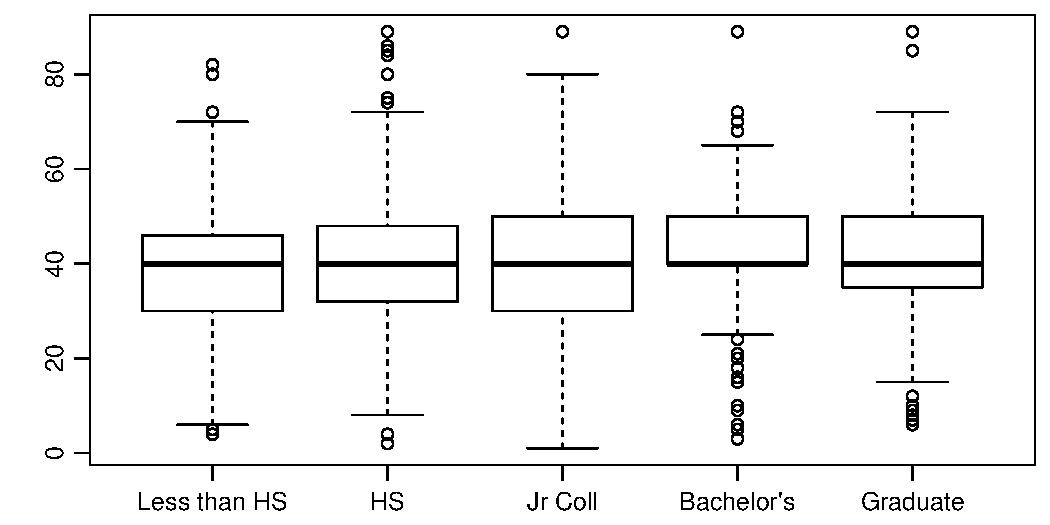
\includegraphics[width=\textwidth]{5-2_diff_two_mean/figures/hrs_edu/hrs_degree_box}
\end{center}

\end{frame}

%%%%%%%%%%%%%%%%%%%%%%%%%%%%%%%%%%%%

\begin{frame}[fragile]
\frametitle{Collapsing levels into two}

\begin{itemize}

\item Say we are only interested the difference between the number of hours worked per week by college and non-college graduates.

\pause

\item Then we combine the levels of education into two:
\begin{itemize}
\item \texttt{hs or lower} $\leftarrow$ less than high school or high school
\item \texttt{coll or higher} $\leftarrow$ junior college, bachelor's, and graduate
\end{itemize}

\end{itemize}

\end{frame}
%%%%%%%%%%%%%%%%%%%%%%%%%%%%%%%%%%%%

\begin{frame}
\frametitle{Exploratory analysis - another look}

\begin{center}
\begin{tabular}{lccc}
\hline
  		& $\bar{x}$ 	& $s$	& $n$ \\
\hline
coll or higher	& 41.8		& 15.14	& 505 \\
hs or lower	& 39.4		& 15.12	& 667 \\
\hline
\end{tabular}
$\:$ \\
\vspace{0.5cm}
$\:$ \\
\includegraphics[width=0.7\textwidth]{5-2_diff_two_mean/figures/hrs_edu/hrs_edu_hist}
\end{center}

\end{frame}

%%%%%%%%%%%%%%%%%%%%%%%%%%%%%%%%%%%

\begin{frame}
\frametitle{Parameter and point estimate}

\dq{We want to construct a 95\% confidence interval for the average difference between the number of hours worked per week by Americans with a college degree and those with a high school degree or lower. What are the parameter of interest and the point estimate?}

\pause

\begin{itemize}

\item \hl{Parameter of interest:} Average difference between the number of hours worked per week by \red{all}  Americans with a college degree and those with a high school degree or lower.
\[ \mu_{coll} - \mu_{hs} \]

\pause

\item \hl{Point estimate:} Average difference between the number of hours worked per week by \red{sampled}  Americans with a college degree and those with a high school degree or lower.
\[ \bar{x}_{coll} - \bar{x}_{hs} \]

\end{itemize}

\end{frame}

%%%%%%%%%%%%%%%%%%%%%%%%%%%%%%%%%%%

\begin{frame}[shrink]
\frametitle{Checking assumptions \& conditions}

\begin{enumerate}

\item \hl{Independence within groups: }
\begin{itemize}
\item Both the college graduates and those with HS degree or lower are sampled randomly.
\pause
\item 505 $<$ 10\% of all college graduates and 667 $<$ 10\% of all students with a high school degree or lower.
\end{itemize}
\pause
We can assume that the number of hours worked per week by one college graduate in the sample is independent of another, and the number of hours worked per week by someone with a HS degree or lower in the sample is independent of another as well.

\pause

\item \hl{Independence between groups: } \red{$\leftarrow$ new!} \\
Since the sample is random, the college graduates in the sample are independent of those with a HS degree or lower.

\pause

\item \hl{Sample size / skew:} \\
Both distributions look reasonably symmetric, and the sample sizes are at least 30, therefore we can assume that the sampling distribution of number of hours worked per week by college graduates and those with HS degree or lower are nearly normal. Hence the sampling distribution of the average difference will be nearly normal as well.

\end{enumerate}

\end{frame}

%%%%%%%%%%%%%%%%%%%%%%%%%%%%%%%%%%%

\begin{frame}
\frametitle{Confidence interval for difference between two means}

\begin{itemize}

\item All confidence intervals have the same form:
\[ \textcolor{orange}{point~estimate \pm ME} \]

\pause

\item And all $ \textcolor{orange}{ME = critical~value \times SE~of~point~estimate}$

\pause

\item In this case the point estimate is $\bar{x}_1 - \bar{x}_2$

\pause

\item Since the sample sizes are large enough, the critical value is $z^\star$

\pause

\item So the only new concept is the standard error of the difference between two means...

\end{itemize}

\pause

\formula{Standard error of the difference between two sample means}
{
\[ SE_{(\bar{x}_1 - \bar{x}_2)} = \sqrt{ \frac{s_1^2}{n_1} + \frac{s_2^2}{n_2} } \]
}

\end{frame}

%%%%%%%%%%%%%%%%%%%%%%%%%%%%%%%%%%%

\begin{frame}
\frametitle{Let's put things in context}

\dq{Calculate the standard error of the average difference between the number of hours worked per week by college graduates and those with a HS degree or lower.}

\twocol{0.5}{0.5}
{
\begin{tabular}{lccc}
\hline
			& $\bar{x}$ 	& $s$	& $n$ \\
\hline
coll or higher	& 41.8		& 15.14	& 505 \\
hs or lower	& 39.4		& 15.12	& 667 \\
\hline
\end{tabular}
}
{
\pause
\begin{eqnarray*}
SE_{(\bar{x}_{coll} - \bar{x}_{hs})} &=& \sqrt{ \frac{s_{coll}^2}{n_{coll}} + \frac{s_{hs}^2}{n_{hs}} } \\
\pause
&=& \sqrt{ \frac{15.14^2}{505} + \frac{15.12^2}{667} } \\
\pause
&=& 0.89
\end{eqnarray*}
}

\end{frame}

%%%%%%%%%%%%%%%%%%%%%%%%%%%%%%%%%%%

\begin{frame}
\frametitle{Confidence interval for the difference (cont.)}

\dq{Estimate (using a 95\% confidence interval) the average difference between the number of hours worked per week by Americans with a college degree and those with a high school degree or lower. 
\[ \bar{x}_{coll} = 41.8 \qquad \bar{x}_{hs} = 39.4 \qquad SE_{(\bar{x}_{coll} - \bar{x}_{hs})} = 0.89 \]}

\pause

\begin{eqnarray*}
(\bar{x}_{coll} - \bar{x}_{hs}) \pm z^\star \times SE_{(\bar{x}_{coll} - \bar{x}_{hs})} &=& (41.8 - 39.4) \pm 1.96 \times 0.89 \\
\pause
&=& 2.4 \pm 1.74 \\
\pause
&=& (0.66, 4.14)
\end{eqnarray*}


\end{frame}

%%%%%%%%%%%%%%%%%%%%%%%%%%%%%%%%%%%

\begin{frame}
\frametitle{Interpretation of a confidence interval for the difference}

\pq{Which of the following is the \underline{best} interpretation of the confidence interval we just calculated?}

\begin{enumerate}[(a)]
\item The difference between the average number of hours worked per week by college grads and those with a HS degree or lower is between 0.66 and 4.14 hours.
\solnMult{College grads work on average of 0.66 to 4.14 hours more per week than those with a HS degree or lower.}
\item College grads work on average 0.66 hours less to 4.14 hours more per week than those with a HS degree or lower.
\item College grads work on average 0.66 to 4.14 hours less per week than those with a HS degree or lower.
\end{enumerate}

\end{frame}

%%%%%%%%%%%%%%%%%%%%%%%%%%%%%%%%%%%

\begin{frame}
\frametitle{Reality check}

\dq{Do these results sound reasonable? Why or why not?}

\end{frame}


%%%%%%%%%%%%%%%%%%%%%%%%%%%%%%%%%%%

\subsection{Hypothesis tests for differences of means}

%%%%%%%%%%%%%%%%%%%%%%%%%%%%%%%%%%%

\begin{frame}
\frametitle{Setting the hypotheses}

\dq{What are the hypotheses for testing if there is a difference between the average number of hours worked per week by college graduates and those with a HS degree or lower?}

\pause

\begin{itemize}
\item[$H_0$:] $\mu_{coll} = \mu_{hs}$  \\
{\small There is no difference in the average number of hours worked per week by college graduates and those with a HS degree or lower. Any observed difference between the sample means is due to natural sampling variation (chance).}
\pause
\item[$H_A$:] $\mu_{coll} \neq \mu_{hs}$  \\
{\small There is a difference in the average number of hours worked per week by college graduates and those with a HS degree or lower.}
\end{itemize}

\end{frame}

%%%%%%%%%%%%%%%%%%%%%%%%%%%%%%%%%%%

\begin{frame}[shrink]
\frametitle{Calculating the test-statistic and the p-value}

\begin{itemize}
\item[$H_0$:] $\mu_{coll} = \mu_{hs} \rightarrow$ \red{$\mu_{coll} - \mu_{hs} = 0$} \\
\item[$H_A$:] $\mu_{coll} \neq \mu_{hs} \rightarrow \mu_{coll} - \mu_{hs} \ne 0$  \\
\item[]
\item[] $\bar{x}_{coll} - \bar{x}_{hs} = 2.4$, $SE_(\bar{x}_{coll} - \bar{x}_{hs}) = 0.89$
\end{itemize}


\pause

\twocol{0.5}{0.5}
{
\begin{center}
\includegraphics[width=\textwidth]{5-2_diff_two_mean/figures/hrs_edu/hrs_norm}
\end{center}
}
{
\pause
\small{
\begin{eqnarray*}
Z &=& \frac{(\bar{x}_{coll} - \bar{x}_{hs}) - 0}{ SE_{(\bar{x}_{coll} - \bar{x}_{hs})} } \\
\pause
&=& \frac{2.4}{0.89} = 2.70 \\
\pause
upper~tail &=&  1 -  0.9965 = 0.0035 \\
\pause
p-value &=& 2 \times 0.0035 = 0.007
\end{eqnarray*}
}
}

\end{frame}

%%%%%%%%%%%%%%%%%%%%%%%%%%%%%%%%%%%

\begin{frame}
\frametitle{Conclusion of the test}

\pq{Which of the following is correct based on the results of the hypothesis test we just conducted?}

{\small
\begin{enumerate}[(a)]
\item There is a 0.7\% chance that there is no difference between the average number of hours worked per week by college graduates and those with a HS degree or lower.
\solnMult{Since the p-value is low, we reject $H_0$. The data provide convincing evidence of a difference between the average number of hours worked per week by college graduates and those with a HS degree or lower.}
\item Since we rejected $H_0$, we may have made a Type 2 error.
\item Since the p-value is low, we fail to reject $H_0$. The data do not provide convincing evidence of a difference between the average number of hours worked per week by college graduates and those with a HS degree or lower.
\end{enumerate}
}

\end{frame}

%%%%%%%%%%%%%%%%%%%%%%%%%%%%%%%%%%%%
\input{5-3_one_t/5-3_one_t}
%%%%%%%%%%%%%%%%%%%%%%%%%%%%%%%%%%%%

\section{The $t$ distribution for the difference of two means}

%%%%%%%%%%%%%%%%%%%%%%%%%%%%%%%%%%%%

\begin{frame}
\frametitle{Diamonds}

\begin{itemize}

\item Weights of diamonds are measured in carats. 

\item 1 carat = 100 points, 0.99 carats = 99 points, etc.

\item The difference between the size of a 0.99 carat diamond and a 1 carat diamond is undetectable to the naked human eye, but does the price of a 1 carat diamond tend to be higher than the price of a 0.99 diamond?

\item We are going to test to see if there is a difference between the average prices of 0.99 and 1 carat diamonds.

\item In order to be able to compare equivalent units, we divide the prices of 0.99 carat diamonds by 99 and 1 carat diamonds by 100, and compare the average point prices.

\end{itemize}

\hfill \includegraphics[width=0.3\textwidth]{5-4_two_t/figures/diamonds/diamond}

\end{frame}

%%%%%%%%%%%%%%%%%%%%%%%%%%%%%%%%%%%

\begin{frame}[fragile]
\frametitle{Data}

\begin{center}
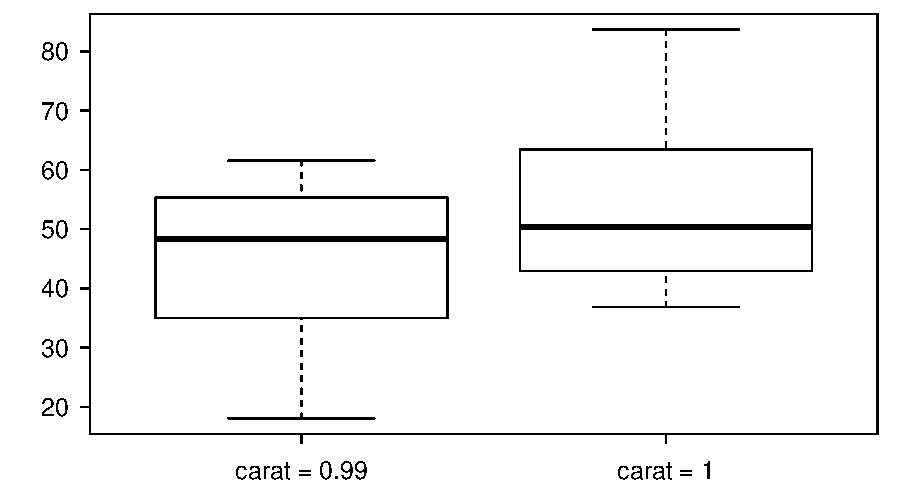
\includegraphics[width=0.7\textwidth]{5-4_two_t/figures/diamonds/diamondBox}
\end{center}

{\small
\begin{center}
\begin{tabular}{l | c | c}
		& {\footnotesize \hl{0.99 carat}} &  {\footnotesize \hl{1 carat}}  \\
		& pt99	& pt100 \\
\hline
$\bar{x}$	& 44.50		& 53.43 \\
$s$		& 13.32		& 12.22 \\
$n$		& 23			& 30
\end{tabular}
\end{center}
}

\vfill

\rule{2.5cm}{0.25pt} \\
{\tiny These data are a random sample from the \texttt{diamonds} data set in \texttt{ggplot2} R package.}

\end{frame}

%%%%%%%%%%%%%%%%%%%%%%%%%%%%%%%%%%%

\begin{frame}
\frametitle{Parameter and point estimate}

\begin{itemize}

\item \hl{Parameter of interest:} Average difference between the point prices of \red{all} 0.99 carat and 1 carat diamonds.
\[ \mu_{pt99} - \mu_{pt100} \]

$\:$ \\

\pause

\item \hl{Point estimate:} Average difference between the point prices of \red{sampled}  0.99 carat and 1 carat diamonds.
\[ \bar{x}_{pt99} - \bar{x}_{pt100} \]

\end{itemize}

\end{frame}

%%%%%%%%%%%%%%%%%%%%%%%%%%%%%%%%%%%

\begin{frame}
\frametitle{Hypotheses}

\pq{Which of the following is the correct set of hypotheses for testing if the average point price of 1 carat diamonds ($_{pt100}$) is higher than the average point price of 0.99 carat diamonds ($_{pt99}$)?}

\begin{enumerate}[(a)]

\item  \mathhl{H_0:} $\mu_{pt99} = \mu_{pt100}$ \\
\mathhl{H_A:} $\mu_{pt99} \ne \mu_{pt100}$

\item  \mathhl{H_0:} $\mu_{pt99} = \mu_{pt100}$ \\
\mathhl{H_A:} $\mu_{pt99} > \mu_{pt100}$

\solnMult{  \mathhl{H_0:} $\mu_{pt99} = \mu_{pt100}$ \\
\mathhl{H_A:} $\mu_{pt99} < \mu_{pt100}$ }

\item  \mathhl{H_0:} $\bar{x}_{pt99} = \bar{x}_{pt100}$ \\
\mathhl{H_A:} $\bar{x}_{pt99} < \bar{x}_{pt100}$

\end{enumerate}

\end{frame}

%%%%%%%%%%%%%%%%%%%%%%%%%%%%%%%%%%%

\begin{frame}
\frametitle{Conditions}

\pq{Which of the following does \underline{not} need to be satisfied in order to conduct this hypothesis test using theoretical methods?}

\begin{enumerate}[(a)]

\item Point price of one 0.99 carat diamond in the sample should be independent of another, and the point price of one 1 carat diamond should independent of another as well.

\item Point prices of 0.99 carat and 1 carat diamonds in the sample should be independent.

\item Distributions of point prices of 0.99 and 1 carat diamonds should not be extremely skewed.

\solnMult{Both sample sizes should be at least 30.}

\end{enumerate}

\end{frame}

%%%%%%%%%%%%%%%%%%%%%%%%%%%%%%%%%%%%

\subsection{Sampling distribution for the difference of two means}

%%%%%%%%%%%%%%%%%%%%%%%%%%%%%%%%%%%%

\begin{frame}
\frametitle{Test statistic}

\formula{Test statistic for inference on the difference of two small sample means}
{The test statistic for inference on the difference of two small sample means ($n_1 < 30$ and/or $n_2 < 30$) mean is the $T$ statistic.
\[ T_{df} = \frac{\text{point estimate} - \text{null value}}{SE} \]
where 
\[ SE = \sqrt{ \frac{s_1^2}{n_1} + \frac{s_2^2}{n_2} } \qquad \text{ and } \qquad df = min(n_1 - 1, n_2 - 1) \]
}

\Note{The calculation of the $df$ is actually much more complicated. For simplicity we'll use the above formula to \underline{estimate} the true $df$ when conducting the analysis by hand.}

\end{frame}

%%%%%%%%%%%%%%%%%%%%%%%%%%%%%%%%%%%%

\subsection{Hypothesis testing for the difference of two means}

%%%%%%%%%%%%%%%%%%%%%%%%%%%%%%%%%%%%

\begin{frame}
\frametitle{Test statistic (cont.)}

{\small
\begin{center}
\begin{tabular}{l | c | c}
		& {\footnotesize \hl{0.99 carat}} &  {\footnotesize \hl{1 carat}}  \\
		& pt99	& pt100 \\
\hline
$\bar{x}$	& 44.50		& 53.43 \\
$s$		& 13.32		& 12.22 \\
$n$		& 23			& 30
\end{tabular}
\end{center}
}

\hl{in context...}

\pause

{\small
\begin{eqnarray*}
T &=& \frac{\text{point estimate} - \text{null value} }{SE} \\
\pause
&=& \frac{(44.50 - 53.43) - 0}{ \sqrt{\frac{13.32^2}{23} + \frac{12.22^2}{30} }} \\
\pause
&=& \frac{-8.93}{3.56} \\
\pause
&=& -2.508
\end{eqnarray*}
}

\end{frame}

%%%%%%%%%%%%%%%%%%%%%%%%%%%%%%%%%%%%

\begin{frame}
\frametitle{Test statistic (cont.)}

\pq{Which of the following is the correct $df$ for this hypothesis test?}

\twocol{0.3}{0.7}
{
\begin{enumerate}[(a)]
\solnMult{ 22 }
\item 23
\item 30
\item 29
\item 52
\end{enumerate}
}
{
\soln{\only<2>{
\red{$\rightarrow df = min(n_{pt99} - 1, n_{pt100} - 1)$ \\
$= min(23 - 1, 30 - 1)$ \\
$= min(22,29) = 22$} \\
\vspace{1cm}
}}}

\end{frame}

%%%%%%%%%%%%%%%%%%%%%%%%%%%%%%%%%%%%

\begin{frame}
\frametitle{p-value}

\pq{Which of the following is the correct p-value for this hypothesis test?}

\[ T = -2.508 \qquad \only<1-2 | handout:0>{df = 22} \] 

\twocol{0.42}{0.58}
{
\begin{enumerate}[(a)]
\item between 0.005 and 0.01
\solnMult{between 0.01 and 0.025}
\item between 0.02 and 0.05
\item between 0.01 and 0.02
\end{enumerate}
}
{
\only<1>{
{\footnotesize
\begin{tabular}{r | r r  r r r}
\hline
one tail & \hspace{1.5mm}  0.100 & \hspace{1.5mm} 0.050 & \hspace{1.5mm} {0.025} & \hspace{1.5mm} {0.010} & \hspace{1.5mm} 0.005  \\
two tails & 0.200 & 0.100 & 0.050 & 0.020 & 0.010 \\
\hline
df \hfill 21  &  {  1.32} & {  1.72} & {  2.08} & {  2.52} & {  2.83}  \\ 
22  &  {  1.32} & {  1.72} & {  2.07} & {  2.51} & {  2.82}  \\ 
23  &  {  1.32} & {  1.71} & {  2.07} & {  2.50} & {  2.81}  \\ 
24  &  {  1.32} & {  1.71} & {  2.06} & {  2.49} & {  2.80}  \\ 
25  &  {  1.32} & {  1.71} & {  2.06} & {  2.49} & {  2.79}  \\ 
\hline
\end{tabular}
}
}

\only<2|handout:0>{
{\footnotesize
\begin{tabular}{r | r r  >{\columncolor[gray]{.6}[.5\tabcolsep]}r  >{\columncolor[gray]{.6}[.5\tabcolsep]}r r}
\hline
one tail & \hspace{1.5mm}  0.100 & \hspace{1.5mm} 0.050 & \hspace{1.5mm} \red{0.025} & \hspace{1.5mm} \red{0.010} & \hspace{1.5mm} 0.005  \\
two tails & 0.200 & 0.100 & 0.050 & 0.020 & 0.010 \\
\hline
df \hfill 21  &  {  1.32} & {  1.72} & {  2.08} & {  2.52} & {  2.83}  \\ 
  \rowcolor[gray]{.6}
22  &  {  1.32} & {  1.72} & \red{  2.07} & \red{  2.51} & {  2.82}  \\ 
23  &  {  1.32} & {  1.71} & {  2.07} & {  2.50} & {  2.81}  \\ 
24  &  {  1.32} & {  1.71} & {  2.06} & {  2.49} & {  2.80}  \\ 
25  &  {  1.32} & {  1.71} & {  2.06} & {  2.49} & {  2.79}  \\ 
\hline
\end{tabular}
}
}}

\end{frame}

%%%%%%%%%%%%%%%%%%%%%%%%%%%%%%%%%%%%

\begin{frame}
\frametitle{Synthesis}

\dq{What is the conclusion of the hypothesis test? How (if at all) would this conclusion change your behavior if you went diamond shopping?}


\soln{\only<2>{
\begin{itemize}
\item p-value is small so reject $H_0$. The data provide convincing evidence to suggest that the point price of 0.99 carat diamonds is lower than the point price of 1 carat diamonds.
\item Maybe buy a 0.99 carat diamond? It looks like a 1 carat, but is significantly cheaper.
\end{itemize}
}}

\end{frame}

%%%%%%%%%%%%%%%%%%%%%%%%%%%%%%%%%%%%

\subsection{Confidence intervals for the difference of two means}

%%%%%%%%%%%%%%%%%%%%%%%%%%%%%%%%%%%%

\begin{frame}
\frametitle{Equivalent confidence level}

\pq{What is the equivalent confidence level for a one-sided hypothesis test at $\alpha = 0.05$?}


\twocol{0.3}{0.7}{
\begin{enumerate}[(a)]

\solnMult{90\%}

\item 92.5\%

\item 95\%

\item 97.5\%

\end{enumerate}
}
{
\soln{\only<2>{
\includegraphics[width=\textwidth]{5-4_two_t/figures/middle90/middle90}
}}
}

\end{frame}

%%%%%%%%%%%%%%%%%%%%%%%%%%%%%%%%%%%%

\begin{frame}
\frametitle{Critical value}

\pq{What is the appropriate $t^\star$ for a confidence interval for the average difference between the point prices of 0.99 and 1 carat diamonds?}

\begin{enumerate}[(a)]
\item 1.32
\solnMult{1.72}
\item 2.07
\item 2.82
\end{enumerate}

\only<1>{
{\small
\begin{center}
\begin{tabular}{r | r r r r r}
\hline
one tail & \hspace{1.5mm}  0.100 & \hspace{1.5mm} {0.050} & \hspace{1.5mm} {0.025} & \hspace{1.5mm} {0.010} & \hspace{1.5mm} 0.005  \\
two tails & 0.200 & 0.100 & 0.050 & 0.020 & 0.010 \\
\hline
df \hfill 21  &  {  1.32} & {  1.72} & {  2.08} & {  2.52} & {  2.83}  \\ 
22  &  {  1.32} & {  1.72} & {  2.07} & {  2.51} & {  2.82}  \\ 
23  &  {  1.32} & {  1.71} & {  2.07} & {  2.50} & {  2.81}  \\ 
24  &  {  1.32} & {  1.71} & {  2.06} & {  2.49} & {  2.80}  \\ 
25  &  {  1.32} & {  1.71} & {  2.06} & {  2.49} & {  2.79}  \\ 
\end{tabular}
\end{center}
}}

\only<2|handout:0>{
\begin{center}
{\small
\begin{tabular}{r | r >{\columncolor[gray]{.6}[.5\tabcolsep]}r r  r r}
\hline
one tail & \hspace{1.5mm}  0.100 & \hspace{1.5mm} {0.050} & \hspace{1.5mm} {0.025} & \hspace{1.5mm} {0.010} & \hspace{1.5mm} 0.005  \\
two tails & 0.200 & \red{0.100} & 0.050 & 0.020 & 0.010 \\
\hline
df \hfill 21  &  {  1.32} & {  1.72} & {  2.08} & {  2.52} & {  2.83}  \\ 
  \rowcolor[gray]{.6}
22  &  {  1.32} & \red{  1.72} & {  2.07} & {  2.51} & {  2.82}  \\ 
23  &  {  1.32} & {  1.71} & {  2.07} & {  2.50} & {  2.81}  \\ 
24  &  {  1.32} & {  1.71} & {  2.06} & {  2.49} & {  2.80}  \\ 
25  &  {  1.32} & {  1.71} & {  2.06} & {  2.49} & {  2.79}  \\ 
\hline
\end{tabular}
}
\end{center}
}


\end{frame}

%%%%%%%%%%%%%%%%%%%%%%%%%%%%%%%%%%%%

\begin{frame}
\frametitle{Confidence interval}

\dq{Calculate the interval, and interpret it in context.}

\pause

\soln{
\[ \text{point estimate} \pm ME \]
\pause
\begin{eqnarray*}
(\bar{x}_{pt99} - \bar{x}_{pt1}) \pm t^\star_{df} \times SE &=& (44.50 - 53.43) \pm 1.72 \times 3.56 \\
\pause
&=& -8.93 \pm  6.12 \\
\pause
&=& (-15.05, -2.81)
\end{eqnarray*}
\pause
We are 90\% confident that the average point price of a 0.99 carat diamond is \$15.05 to \$2.81 lower than the average point price of a 1 carat diamond.
}

\end{frame}

%%%%%%%%%%%%%%%%%%%%%%%%%%%%%%%%%%%%

\subsection{Recap}

%%%%%%%%%%%%%%%%%%%%%%%%%%%%%%%%%%%%

\begin{frame}
\frametitle{Recap: Inference using difference of two small sample means}

\begin{itemize}

\item If $n_1 < 30$ and/or $n_2 < 30$, difference between the sample means follow a $t$ distribution with $SE = \sqrt{ \frac{s_1^2}{n_1} + \frac{s_2^2}{n_1} }$.

\pause

\item Conditions: 
\begin{itemize}
\item independence within groups (often verified by a random sample, and if sampling without replacement, $n < $ 10\% of population)
\item independence between groups
\item  $n_1 < 30$ and/or $n_2 < 30$ and no extreme skew in either group
\end{itemize}

\pause

\item Hypothesis testing: 
\[ T_{df} = \frac{\text{point estimate} - \text{null value}}{SE}\text{, where }df = min(n_1 - 1, n_2 - 1) \]

\pause

\item Confidence interval:
\[ \text{point estimate} \pm t_{df}^\star \times SE \]

\end{itemize}

\end{frame}

%%%%%%%%%%%%%%%%%%%%%%%%%%%%%%%%%%%

\input{5-5_anova/5-5_anova}


%%%%%%%%%%%%%%%%%%%%%%%%%%%%%%%%%%%%

\end{document}